\documentclass{article}
\usepackage{iko42360}
\usepackage{graphicx} % for pdf, bitmapped graphics files
\graphicspath{{./fig/}}
\DeclareGraphicsExtensions{.pdf,.jpeg,.png}
\usepackage{subfigure}
\usepackage[us,12hr]{datetime} % `us' makes \today behave as usual in TeX/LaTeX

\begin{lecture}{1}{Probabilistic Robotics: Introduction}{Vektor Dewanto}{04/28/2014}

\section{Introduction}
To begin with, consider a tidying-up {PR-1} robot demo from Stanford~\cite{wyrobek10, 4543527}.
In principle, a robot has to have three basic capabilities, namely: mobility, perception and manipulation.
The field of robotics is so broad, ranging from hardware to sofware.
The hardware includes actuators, sensors, controllers and locomotion; putting them altogether, we obtain the so-called ``platform'', e.g. {UBR-1}, Nao, ASIMO.
The sofware can be divided into two big groups: lower and higher levels.
The former covers speed controls, position controls, attitude controls, etc.
Whereas, higher level sofware embraces the field of artificial intelligence, which mainly consists of planning, learning and probabilistics (to deal with uncertainty).
It is worth to mention that the limiting factor in robotics today is more about software.
Building autonomous robot programs is really hard because the variability that the robots have to cope with in the real world.
A good program should be general enough; making hardcoded/scripted code less pervasive.

In robotics, the probabilistic framework is required to mathematically represent and utilize uncertainty.
The uncertainty comes from five major sources~\cite{Thrun:2005:PR}, i.e. environments, computations, models, observations and actions.
Environments are naturally stochastics, for example, the road's condition for self-driving cars is way too uncertain: pedestrian crossing, wheather, traffic, to name a few.
Robots are formed by mechanical stuff that suffers from wear and tear as they operate.
As a result, their physical models become less and less representative, which eventually introduce some degree of uncertainty.
Furthermore, the computations always approximate the continuous values of the real world.
The uncertainty from observations and actions is due to imperfect sensors and actuators.
It is so significant that we will investigate first.

This class assumes that you have mastered some probability knowledge.
It includes topics about random variables, marginal and joint and conditional probabilities, probability distributions, probability density functions, the theorem of total probability, Bayes formula, etc.

\section{The Markov Assumption}
Let $\boldsymbol{u}$ and $\boldsymbol{z}$ denote the robot's action (control) and observation (measurement), respectively.
Let $\boldsymbol{x}$ denotes the state that we want to estimate, e.g. robot's positions in the task of robot localization.
The interaction and evolution among the states, actions and observation can be modelled using the dynamic Bayes network as shown in figure~\ref{fig:bayes_network}.

Moreover, let assume that the state~$\boldsymbol{x}$ has the Markov property, meaning that it compactly summarizes the past without degrading the ability to predict the future~\cite{SuttonBarto:98}.
This implies that the past and future data are independent if one knows the current state $\boldsymbol{x}_t$.
Concretely, in reference to figure~\ref{fig:bayes_network}, we compute $p(\boldsymbol{x}_{t+1} | \boldsymbol{x}_t, \boldsymbol{u}_{t+1})$; instead of $p(\boldsymbol{x}_{t+1} | \boldsymbol{x}_{1:t}, \boldsymbol{u}_{1:t+1})$.
Thus, we are said to utilize the Markov assumption that further assumes that the world is static, the probabilistic models (see section~\ref{sec:action_model} and~\ref{sec:perception_model}) are perfect and the noise is independent over time. 

\begin{figure}[!tb]
  \centering
  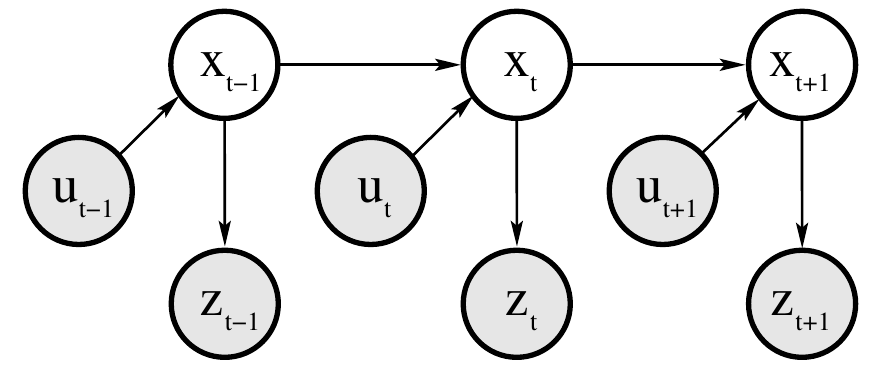
\includegraphics[scale=.33]{bayes_network}
  \caption{The Bayes network that models the interaction and evolution among the states, actions and observation; courtesy of~\cite{Thrun:2005:PR}.}
  \label{fig:bayes_network}
\end{figure}

\section{Action Models} \label{sec:action_model}
The action model is manifested in the form of a transition probability ${p(\boldsymbol{x}_{t} | \boldsymbol{u}_{t}, \boldsymbol{x}_{t-1})}$.
It reads as follows: the probability of the current state~$\boldsymbol{x}_{t}$ given the current control~$\boldsymbol{u}_{t}$ and the past state~$\boldsymbol{x}_{t-1}$.
We will cover in depth about this in the following classes.

Let assume that we use a wheeled robot with odometry motion model.
Consequently, the control (action) is based on the encoder sensor information, e.g. move forward $\boldsymbol{u} = \Delta S = 5~rot$, where $rot$ is a unit representing one full rotation of the wheel.
After several exhaustive experiments, we obtain the error model of the action as depicted in figure~\ref{fig:encoder_err_model}.
\begin{figure}[!tb]
  \centering
  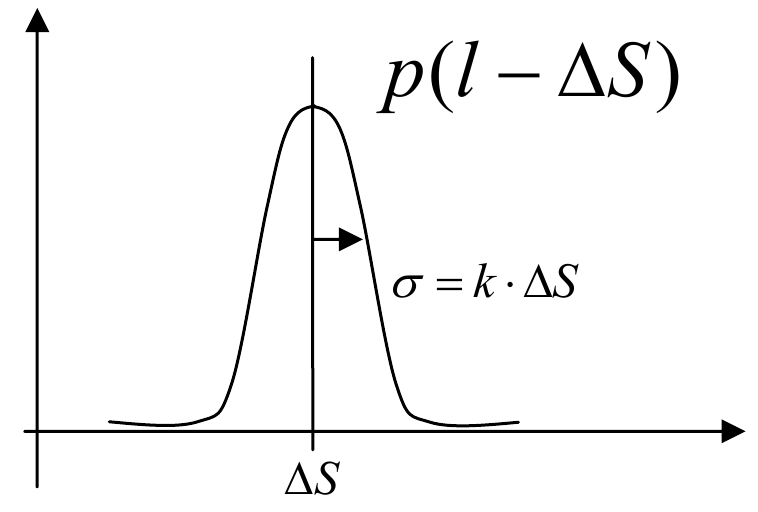
\includegraphics[scale=.5]{encoder_err_model}
  \caption{The odometry error model; courtesy of~\cite{davide09}.}
  \label{fig:encoder_err_model}
\end{figure}

In principle, robot actions increase the uncertainty about the robot's state, e.g. its position for the case of localization.
Figure~\ref{fig:action_increases_uncertainty} and~\ref{fig:action_increases_uncertainty_2} visualize how this happens for the action error model shown in figure~\ref{fig:encoder_err_model}.
Initially, a robot has an absolute certainty about its position at $\boldsymbol{x}_0 = l_0$, which is represented using a dirac distribution.
Afterwards, it executes a sequence of three actions as follows: $\boldsymbol{u}_1 = \Delta S_1$, $\boldsymbol{u}_2 = \Delta S_2 - \Delta S_1$ and $\boldsymbol{u}_3 = \Delta S_3 - \Delta S_2$.
As can be seen, as the robot progresses, the standard deviations of gaussian distributions of $p(l)$ increase.
If it continues to execute the similiar actions, eventually, it will loss information about its localization, in which $p(l)$ has a uniform distribution.

\begin{figure}[!tb]
  \centering
  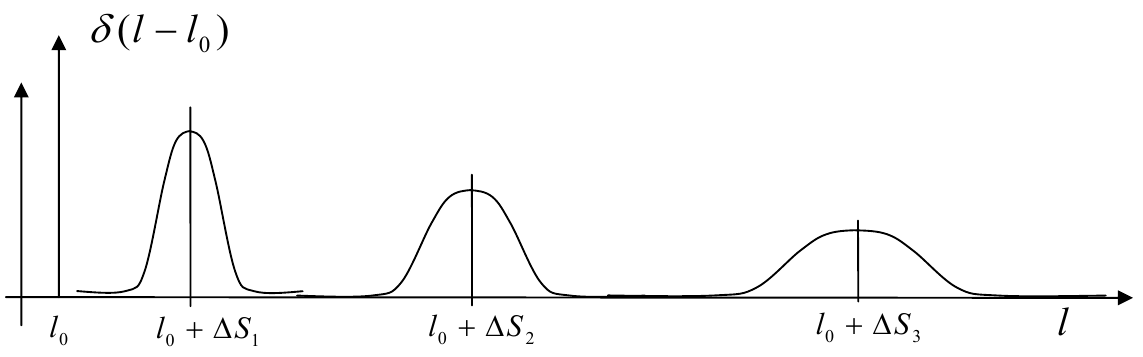
\includegraphics[scale=.5]{action_increases_uncertainty}
  \caption{Robot actions increase uncertainty; courtesy of~\cite{davide09}.}
  \label{fig:action_increases_uncertainty}
\end{figure}

\begin{figure}[!tb]
  \centering
  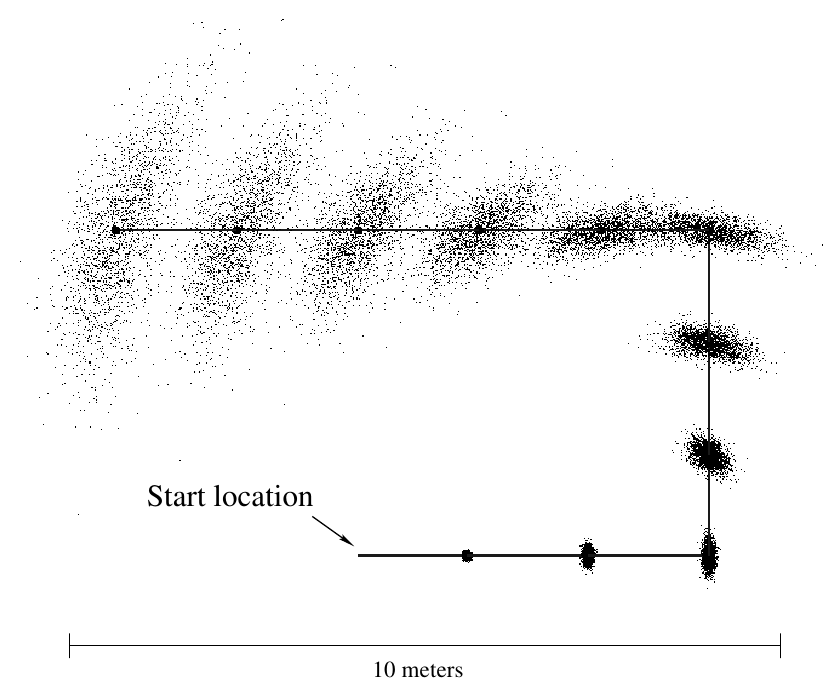
\includegraphics[scale=.5]{action_increases_uncertainty_2}
  \caption{Robot actions increase uncertainty, illustrated using ``particles''; courtesy of~\cite{Thrun:2005:PR}.}
  \label{fig:action_increases_uncertainty_2}
\end{figure}

\section{Perception Models} \label{sec:perception_model}
The perception (or measurement) model is the probability of a measurement (observation) $\boldsymbol{z}_t$ given a state~$\boldsymbol{x}_t$ and a map~$m$, that is $p(\boldsymbol{z}_t |\boldsymbol{x}_t, m)$.
Essentially, the information from sensors refines (increases) the certainty about a state.
As the last section, this topic will be discuss further in the following classes.

Sensors hardly ever return abosolute accurate readings.
For example, sonars (which are quite prevalent in robotics) have three main problems: foreshortening, specular reflection and crosstalk; see figure~\ref{fig:sonar_problem} for more.
In order to handle uncertainty that arises from those problems, the perception model is built based on experiment data.
Concretely, figure~\ref{fig:range_data} dan figure~\ref{fig:measurement_model} shows examples of typical data from range sensors for some true value and the measurement model, respectively.

\begin{figure}[!tb]
  \centering
  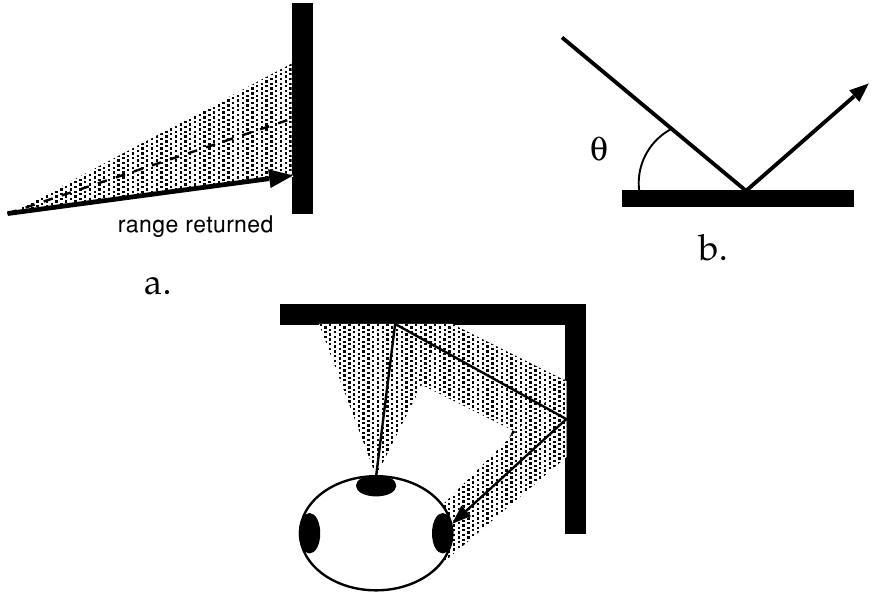
\includegraphics[scale=.5]{sonar_problem}
  \caption{The problems of sonars: a) foreshortening, b) specular reflection and c) crosstalk; courtesy of~\cite{murphy2000introduction}.}
  \label{fig:sonar_problem}
\end{figure}

\begin{figure}[!tb]
  \centering
  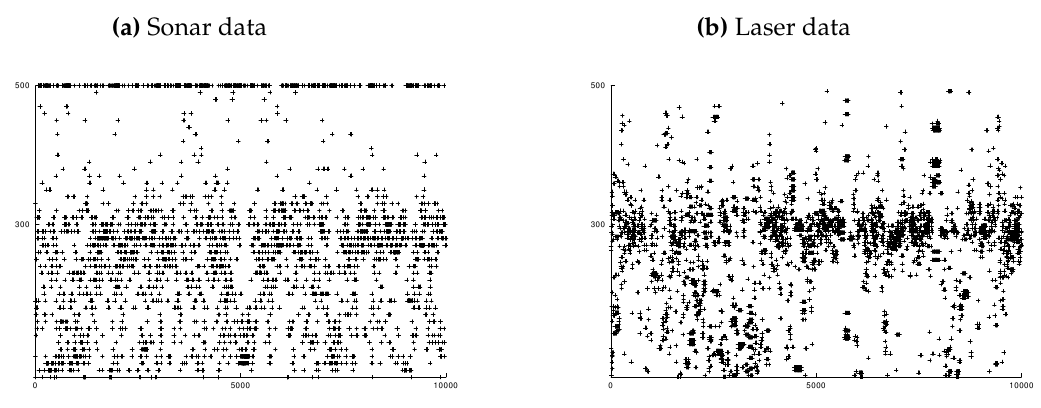
\includegraphics[scale=.6]{range_data}
  \caption{Range data obtained from a sonar and a laser for a true range of 300~cm and a maximum range of 500~cm; courtesy of~\cite{Thrun:2005:PR}.}
  \label{fig:range_data}
\end{figure}

\begin{figure}[!tb]
  \centering
  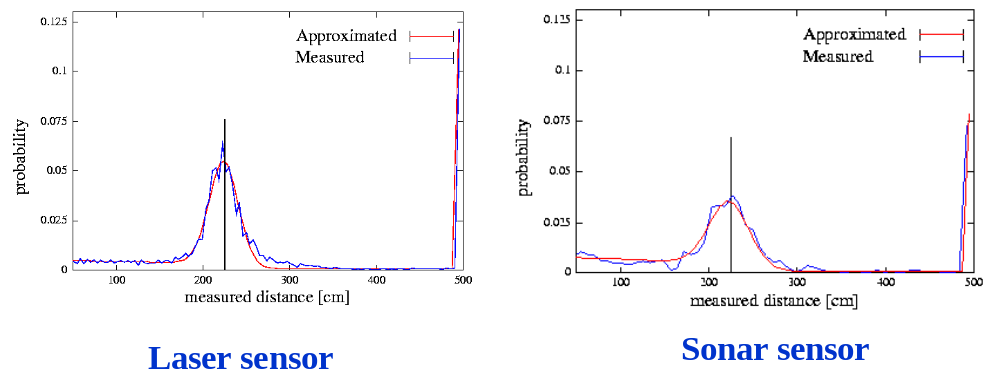
\includegraphics[scale=.6]{measurement_model_2}
  \caption{The measurement model (the red Gaussian distribution curve) based on experiment data (\emph{not} correlated with data in figure~\ref{fig:range_data}); courtesy of~\cite{Thrun:2005:PR}.}
  \label{fig:measurement_model}
\end{figure}

A robot typically employs many sensors; each has its own unique perception model.
As a result, one observation returns $\boldsymbol{z}_t = \{ \boldsymbol{z}_t^1, \boldsymbol{z}_t^2, \ldots, \boldsymbol{z}_t^K \}$, where $K$ is the number of sensors.
If we assume that noise is independent over sensors, then:
\begin{equation*}
    p(\boldsymbol{z}_t |\boldsymbol{x}_t, m) = \prod_{k=1}^K p(\boldsymbol{z}_r^k | \boldsymbol{x}_t, m)
\end{equation*}

\section{The Bayes Filter}
One way to utilize the action and perception models is with the Bayes Filter, which is shown in figure~\ref{fig:bayes_filter}.
In line~3, we do the control update or prediction step or action phase; notice the bar symbol at $\overline{bel}(\boldsymbol{x}_t)$.
More specifically, during action phase, a robot use data from proprioceptive sensors to estimate some state.
Whereas, in line~4, we do the measurement update or perception phase, during which the state estimated on the action phase is updated (refined) with the information from the exteroceptive sensors.
This yields~$bel(\boldsymbol{x}_t)$.

\begin{figure}[!tb]
  \centering
  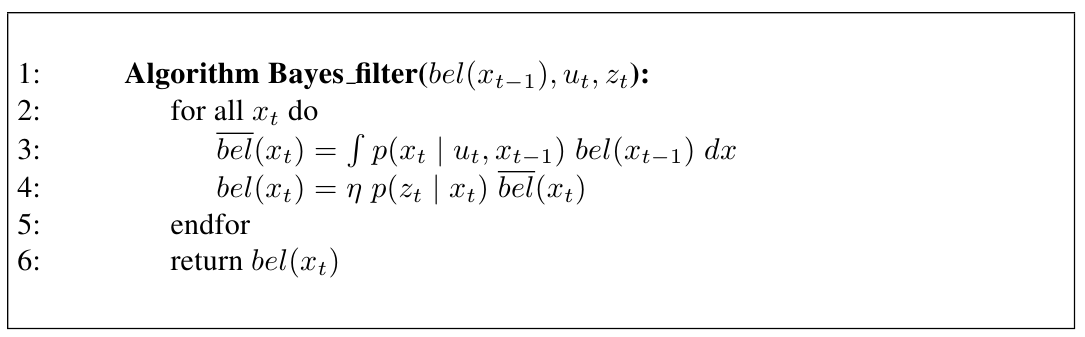
\includegraphics[scale=.5]{bayes_filter}
  \caption{The Bayes Filter algorithm; courtesy of~\cite{Thrun:2005:PR}.}
  \label{fig:bayes_filter}
\end{figure}

As a working example, consider the task of global robot localization illustrated in figure~\ref{fig:global_loc}.
We remark that probabilistic localization requires: (1) an initial probability distribution: $p(\boldsymbol{x}_0)$, (2) an action model: ${p(\boldsymbol{x}_{t} | \boldsymbol{u}_{t}, \boldsymbol{x}_{t-1})}$, (3) a perception model: $p(\boldsymbol{z}_t |\boldsymbol{x}_t, m)$ and (4) a map: $m$.
We cover some details about this localization as follows:
\begin{enumerate}
    \item At ${t=0}$, subfigure~\ref{fig:global_loc}.a, the robot has no information about its localization since this is a global localization problem, in which the robot is not told where it is at $t=0$.
    Consequently, the robot belief $bel(\boldsymbol{x}_0) (=p(\boldsymbol{x}_0))$ has a uniform distribution.
    Notice that $bel(\boldsymbol{x}_t)$ refers to $bel(\boldsymbol{x})$ at time~$t$. 
    \item At ${t=1}$, subfigure~\ref{fig:global_loc}.b, the robot does nothing, $\boldsymbol{u}_1 = \emptyset$, so that $\overline{bel}(\boldsymbol{x}_1) = bel(\boldsymbol{x}_0)$.
    Subsequently, it does the perception phase to obtain $p(\boldsymbol{z}|\boldsymbol{x})$, which is then integrated with $\overline{bel}(\boldsymbol{x_1})$, line~4 in the Bayes algorithm in figure~\ref{fig:bayes_filter}.
    This results in a multimodal gaussian distribution for $bel(\boldsymbol{x}_1)$ with three equal peaks on the door's locations.
    \item At ${t=2}$, subfigure~\ref{fig:global_loc}.c, the robot execute a control to move to the right.
    The last belief, i.e. $bel(\boldsymbol{x}_1)$, is simply shifted to the right to form $\overline{bel}(\boldsymbol{x}_2)$ along with lowered peaks since essentially actions worsens the belief, refer to figure~\ref{fig:encoder_err_model} for the action model.
    \item At ${t=2}$, subfigure~\ref{fig:global_loc}.d, the robot also does the perception phase and use the result to update its $\overline{bel}(\boldsymbol{x}_2)$ to become $bel(\boldsymbol{x}_2)$.
    Now, $bel(\boldsymbol{x}_2)$ has a distinguishable peak in front of the middle door.
    At this point, we can say that the robot has succeeded to localize its position.
    \item At ${t=3}$, subfigure~\ref{fig:global_loc}.e, the robot moves to the right again.
    This surely decrease the belief so that $\overline{bel}(\boldsymbol{x}_3)$ has lower peaks.
    Even so, the highest peak is still superior, meaning that, to some extent of certainty, its location remains localized.
\end{enumerate}

\begin{figure}[!tb]
  \centering
  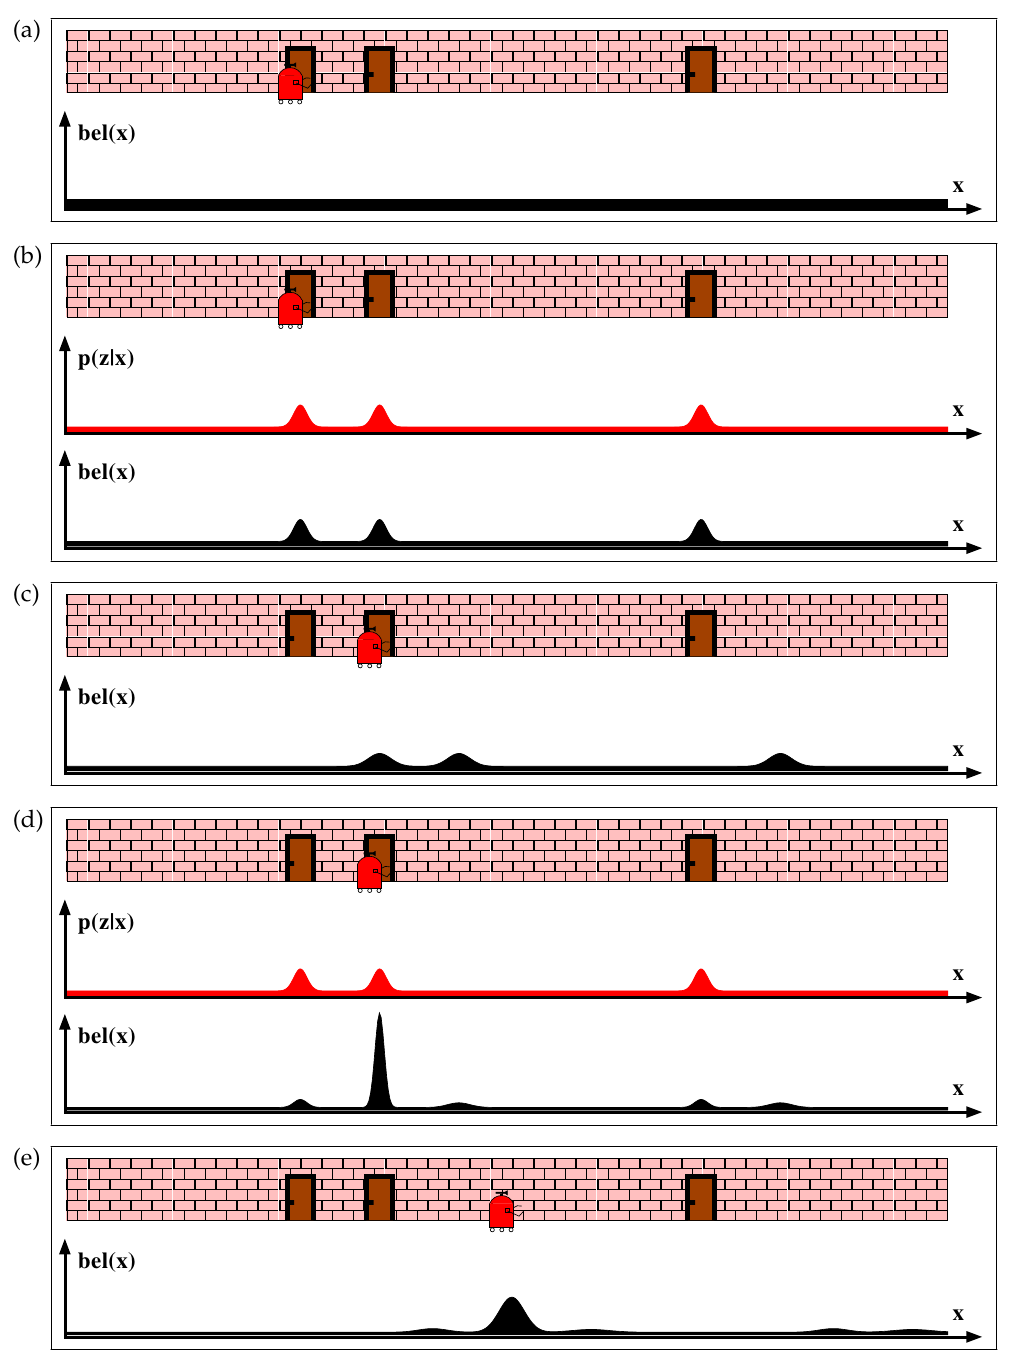
\includegraphics[scale=.55]{global_loc}
  \caption{An illustration of global localization; courtesy of~\cite{Thrun:2005:PR}.}
  \label{fig:global_loc}
\end{figure}

\section{Miscellany}
This was prepared by Vektor, who gratefully acknowledges Dr.~Eng.~Wisnu Jatmiko for such teaching opportunity.
You may contact him at vektor.dewanto@gmail.com.
(compiled on {\ddmmyyyydate\today} at \currenttime)

\bibliographystyle{IEEEtran}
\bibliography{IEEEabrv,ref}

\end{lecture}
\theend
